\section{\texttt{googleVis}}

%----------------------------------------------------------------------

\subsection{Descrição}

\begin{frame}

  \begin{itemize}
  \item Interface R para gráficos \textit{a la} Google Docs SpreadSheets, usa a
    \emph{Google Charts API}.
  \item O mais conhecido desses \textit{charts} é provavelmente o
    \textbf{Motion Chart}, popularizado por Hans Rosling em seu
    \href{??}{TED talk}. INCLUIR UM PRINTSCREEN E O LINK.
  \item Visualizar dados em data frames com gráficos Google sem upload
    no Google Docs.
  \item O resultado é um html com funções JavaScript hopedadas pelo
    Google que é rederizado pelo navegador.
  \item Requer conexão, às vezes flash.
  \end{itemize}

  \begin{itemize}
  \item Autores: Markus Gesmann, Diego de Castillo, Joe Cheng
  \item Lançamento: 03-Dec-2010
  \item Versão: 0.5.9
  \item URL:
    \url{http://cran.r-project.org/web/packages/googleVis/index.html},
    \url{https://github.com/mages/googleVis}
  \end{itemize}
  
\end{frame}

\begin{frame}
  \begin{itemize}
  \item Dado estruturado em \texttt{DataTable}.
  \item Transforma \texttt{data.frame}s em objetos JSON.
  \item Usa o \texttt{RJSONIO} para gerar JSON.
  \item Na versão 0.5.9: COLOCAR AQUI A LISTA... E UM PRINT SCREEN BEM CHAMATIVO.
  \end{itemize}
\end{frame}

%----------------------------------------------------------------------

\subsection{Como usar}
  
\frame{
  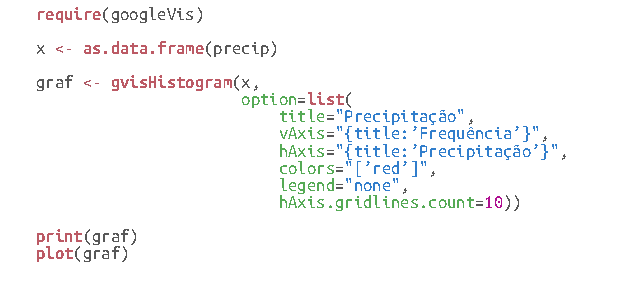
\includegraphics{./tikz/googleVis_gvisHistogram-1.pdf}
}  

\frame{
  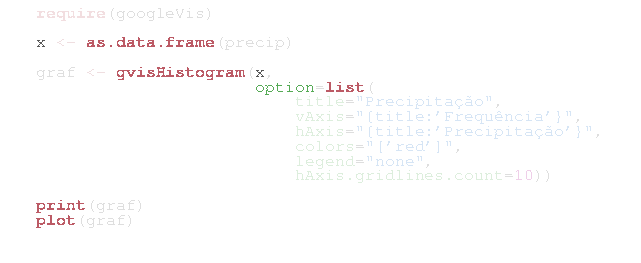
\includegraphics{./tikz/googleVis_gvisHistogram-2.pdf}
}

\frame{
  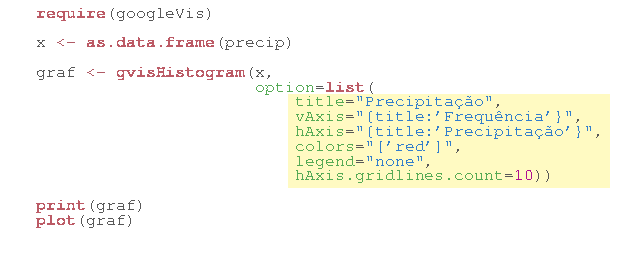
\includegraphics{./tikz/googleVis_gvisHistogram-3.pdf}
}

%----------------------------------------------------------------------

\subsection{Exemplos}

\begin{frame}

 Praticando:
  \begin{enumerate}
  \item \href{run:./R/googleVis/googleVis.R}{R Script googleVis}
  \item \href{run:googleVis.html}{Galeria googleVis IGUIR}
  \end{enumerate}

  \vspace{0.5cm}
  Algumas aplicações com o googleVis:
  \begin{itemize}
  \item \href{http://cran.r-project.org/web/packages/googleVis/vignettes/}{Galeria
      do autor},
  \item \href{http://www.r-bloggers.com/?s=googleVis}{Busca no R
      Bloggers}
  \end{itemize}

\end{frame}
